We define
\begin{align*}
    \omega_s = \frac{\pi^{s/2}}{\Gamma(1 + s/2)},
\end{align*}
in Section \ref{hausdorff_measure}, where $\Gamma$ is Euler gamma function. We want to prove that if $s = n \in \mathbb{N}$, then $\omega_n$ is volume of the unit ball in $\mathbb{R}^n$. First, the Euler gamma function is defined as
\begin{align*}
    \Gamma(x) = \int^\infty_{0} t^{x-1} e^{-t}\, dt, \quad 0 < x <\infty.
\end{align*}
Next, we discuss some properties of the gamma function.

\medskip

\begin{theorem}
~\begin{enumerate}[label=(\alph*)]
    \item $\Gamma(x+1) = x \Gamma(x)$,
    
    \item $\Gamma(n+1) = n!, n \in \mathbb{N}$,
    
    \item $\Gamma(1/2) = \sqrt{\pi}$.
\end{enumerate}
\end{theorem}
\begin{proof}
~\begin{enumerate}[label=(\alph*)]
    \item \begin{align*}
        \Gamma(x+1) & = \int^\infty_{0} t^{x} e^{-t}\, dt = \underbrace{\left(-t^xe^t\right)\Big|^\infty_{t=0}}_{=\,0} + x \int^\infty_{0} t^{x-1} e^{-t}\, dt = x \Gamma(x).
    \end{align*}
    
    \item Since $\displaystyle \Gamma(1) = \int^\infty_0 e^{-t}\, dt = 1$, then
    \begin{align*}
        \Gamma(2) = 1 & \cdot \Gamma(1) = 1, \\
        \Gamma(3) = 2 & \cdot \Gamma(2) = 2, \\
        \Gamma(4) = 3 & \cdot \Gamma(3) = 6,\\
        & \, \vdots \\
        \Gamma(n+1) = n & \cdot \Gamma(n) = n!.
    \end{align*}
    
    \item We need a lemma to prove this part.
    \begin{lemma}\label{lemma_A2}
    The integral of the Gaussian function $f(x) = e^{-x^2}$ is
    $\displaystyle \int^\infty_{-\infty} e^{-x^2}\, dx = \sqrt{\pi}$ or $\displaystyle \int^\infty_0 e^{-x^2}\, dx = \frac{\sqrt{\pi}}{2}$.
    \end{lemma}
    \begin{proof}
    A standard way to compute the Gaussian integral is to make use of the property that\footnote{This proof is provided in Wikipedia: \url{https://en.wikipedia.org/wiki/Gaussian_integral}.}:
    \begin{align*}
        \left(\int^\infty_{-\infty} e^{-x^2}\, dx\right)^2 = \int^\infty_{-\infty} e^{-x^2}\, dx \int^\infty_{-\infty} e^{-y^2}\, dy = \int^\infty_{-\infty} \int^\infty_{-\infty} e^{-(x^2+y^2)}\, dxdy.
    \end{align*}
    Using polar coordinates gives
    \begin{align*}
        \int^\infty_{-\infty} \int^\infty_{-\infty} e^{-(x^2+y^2)}\, dxdy = \int^{2\pi}_0 \int^\infty_0 e^{-r^2} r \, dr d\theta = 2\pi \int^\infty_0 r e^{-r^2} \, dr = 2\pi \left(-\frac{1}{2} e^{-r^2}\right) \Bigg|^\infty_0 = \pi.
    \end{align*}
    \end{proof}
    
    Now for the gamma function, let $t = s^2$, then $\displaystyle \Gamma(x) = 2 \int^\infty_0 s^{2x-1} e^{-s^2}\, ds$. Also by Lemma \ref{lemma_A2}, we have $\displaystyle \Gamma(1/2) = \int^\infty_{-\infty} e^{-s^2}\, ds = \sqrt{\pi}$, which proved the theorem.
\end{enumerate}
\end{proof}

\medskip

\begin{remark}
We can define $\Gamma(x) = \Gamma(x+1) / x$ even if $x < 0$ but $x \notin \mathbb{Z}$. For example, 
\begin{align*}
    \Gamma\left(-\frac{3}{2}\right) = \frac{\Gamma\left(-1/2\right)}{-3/2} = \frac{\Gamma\left(1/2\right)}{3/4} = \frac{4\sqrt{\pi}}{3}.
\end{align*}
Thus, we can extend the gamma function to $x \in (-\infty, \infty) \setminus \{0, -1, -2, \cdots\}$.
\end{remark}

\medskip

\begin{lemma}
$\displaystyle \int^{\pi/2}_0 \sin^n(\theta)\, d\theta = \frac{\sqrt{\pi} \, \Gamma\left(\frac{n+1}{2}\right)}{n \Gamma\left(\frac{n}{2}\right)}$, $n = 1,2,\cdots$.
\end{lemma}
\begin{proof}
Denote the left hand side by $a_n$ and right hand side by $b_n$. For $a_n$,
\begin{align*}
    a_{n+2} & = \int^{\pi/2}_0 \sin^{n+1}(\theta) \sin (\theta)\, d\theta \\
    & = \underbrace{\left( - \sin^{n+1}(\theta) \cos(\theta) \right)\Big|^{\pi/2}_0}_{=\, 0} + (n+1) \int^{\pi/2}_0 \sin^n(\theta) \underbrace{\cos^2(\theta)}_{=\, 1 - \sin^2(\theta)}\, d\theta \\
    & = (n+1)(a_n - a_{n+2}),
\end{align*}
and then
\begin{align*}
    a_{n+2} = \frac{n+1}{n+2}a_n.
\end{align*}

For $b_n$,
\begin{align*}
    b_{n+2} = \frac{\sqrt{\pi} \, \Gamma\left(\frac{n+1}{2} + 1\right)}{(n+2) \Gamma\left(\frac{n}{2} + 1\right)} = \frac{\sqrt{\pi} \frac{n+1}{2} \Gamma\left(\frac{n+1}{2}\right)}{(n+2) \frac{n}{2} \Gamma\left(\frac{n}{2}\right)} = \frac{n+1}{n+2} b_n,
\end{align*}
and then
\begin{align*}
    b_{n+2} = \frac{n+1}{n+2}b_n.
\end{align*}
Also, since $a_1 = b_1 = 1$, $a_2 = b_2 = \pi/4$, the lemma follows.
\end{proof}

\medskip

\begin{theorem}
~\begin{enumerate}[label=(\alph*)]
    \item The volume $\omega_n$ of the unit ball in $\mathbb{R}^n$ equals
    \begin{align*}
        \omega_n = \frac{2\pi^{n/2}}{n \Gamma(n/2)} = \frac{\pi^{n/2}}{\Gamma(n/2 + 1)}.
    \end{align*}
    
    \item The surface area, or $(n-1)$-volume $S_{n-1}$ of boundary sphere $S^{n-1}(0,1)$ equals $n \omega_n$.
\end{enumerate}
\end{theorem}
\begin{proof}
~\begin{enumerate}[label=(\alph*)]
    \item Considering the unit ball in $\mathbb{R}^3$ would be helpful, and the horizontal view is shown below:
    \begin{figure}[H]
        \centering
        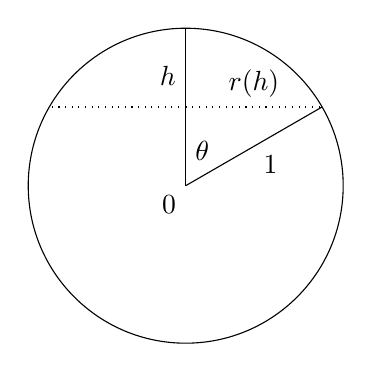
\begin{tikzpicture}[scale=1]
            \draw (0,0) circle (2);
            \draw[-] (0,0)--(1.732,1) node[pos=.5, below right]{$1$};
            \draw[-] (0,0) node[below left]{$0$}--(0, 2) node[pos=.1, above right]{$\theta$} node[pos=.7, left]{$h$};
            \draw[dotted,-] (0,1) -- (1.732,1) node[pos=0.5, above]{$r(h)$};
            \draw[dotted,-] (0,1) -- (-1.732,1);
        \end{tikzpicture}
        \caption{The horizontal view of unit ball in $\mathbb{R}^3$.}
        \label{fig:unit_ball}
    \end{figure}
    We have $r(h) = \sin(\theta)$, and $h = 1 - \cos(\theta)$. Using Fubini's theorem, consider the upper half of the unit ball, we have
    \begin{align*}
        \frac{1}{2}\omega_n & = \int^1_0 \omega_{n-1} r(h)^{n-1} \, dh \\
        & = \omega_{n-1} \int^{\pi/2}_0 \sin^{n-1}(\theta) \underbrace{\sin(\theta)}_{dh}\, d\theta \\
        & = \omega_{n-1} \frac{\sqrt{\pi} \, \Gamma\left(\frac{n+1}{2}\right)}{n \Gamma\left(\frac{n}{2}\right)},
    \end{align*}
    which implies
    \begin{align*}
        \omega_n = \frac{2 \sqrt{\pi}\, \Gamma\left(\frac{n+1}{2}\right)}{n \Gamma\left(\frac{n}{2}\right)} \omega_{n-1}.
    \end{align*}
    If $\displaystyle a_n = \frac{2\pi^{n/2}}{n \Gamma(n/2)}$, then $a_1 = 2 = \omega_1$, and $a_n$ satisfies the same recurrence as $\omega_n$. Thus, $\omega_n = a_n$ for all $n = 1,2,\cdots$.
    
    \item Representing the unit $n$-ball as a union of concentric $(n - 1)$-sphere gives
    \begin{align*}
        \omega_n = \int^1_0 S_{n-1} r^{n-1} \, dr = \frac{1}{n} S_{n-1},
    \end{align*}
    which proves the theorem.
\end{enumerate}
\end{proof}